\section[Logarithmic concentration for polynomials with random signs]{Logarithmic concentration for polynomials\\with random signs}
\label{sec:concentration}\label{sec:layer2}

Section~\ref{sec:radial} reduces root counts to the angular logarithm
$J_N(r)$, so we now show that $J_N(r)$ is close to its Gaussian value
$\log\sigma_N(r)-\gamma/2$. At one angle, and at two separated angles, the
normalized polynomial is close in law to one and to two independent copies
of $G$, which controls how often it is small; logarithmic integrability
controls the rest.
Let $X_r(\theta)=f_N(re^{i\theta})/\sigma_N(r)$, so that
$J_N(r)-\log\sigma_N(r)=\int\log|X_r|\dd\mu$, where $G$ has density
$\pi^{-1}e^{-|z|^2}$ on $\mathbb C$. We fix $K\ge2$ before letting $N$
tend to infinity; exact bounds and degree thresholds are in
Appendix~\ref{sec:constants}.

\begin{theorem}[Concentration of the angular logarithm]
\label{thm:sign-logarithms}
Fix $K\ge2$. For all sufficiently large $N$, uniformly for
$r\in[1-K/N,1+K/N]$,
\begin{align}
 &\Prob\!\left\{
 |J_N(r)-\log\sigma_N(r)+\gamma/2|
       >C(K)N^{-1/16}(\log N)^7\right\}\nonumber\\
 &\qquad\le C(K)N^{-3/8}+N^{-12}
                 +C(K)N^{-3/8}(\log N)^{-12}.
 \label{eq:sign-log-concentration}
\end{align}
\end{theorem}

Here the constants and the degree threshold depend only on $K$.
In particular, these probabilities are summable along $N=j^8$, since there
$N^{-3/8}=j^{-3}$.

Theorem~\ref{thm:sign-logarithms} gives, at every radius of the annulus
$[1-K/N,1+K/N]$, the logarithmic bounds that Lemmas~\ref{lem:annular-mass}
and~\ref{lem:thin-band} require (Corollary~\ref{cor:radial-probability}).
Section~\ref{sec:h1-rademacher} controls the occupation of small disks,
and Section~\ref{sec:log-integrability} adds the logarithmic integrability
of Nazarov--Nishry--Sodin and proves the theorem.

Figure~\ref{fig:angular-logarithm} illustrates the theorem for one nested sequence.

\begin{figure}[t]
\centering
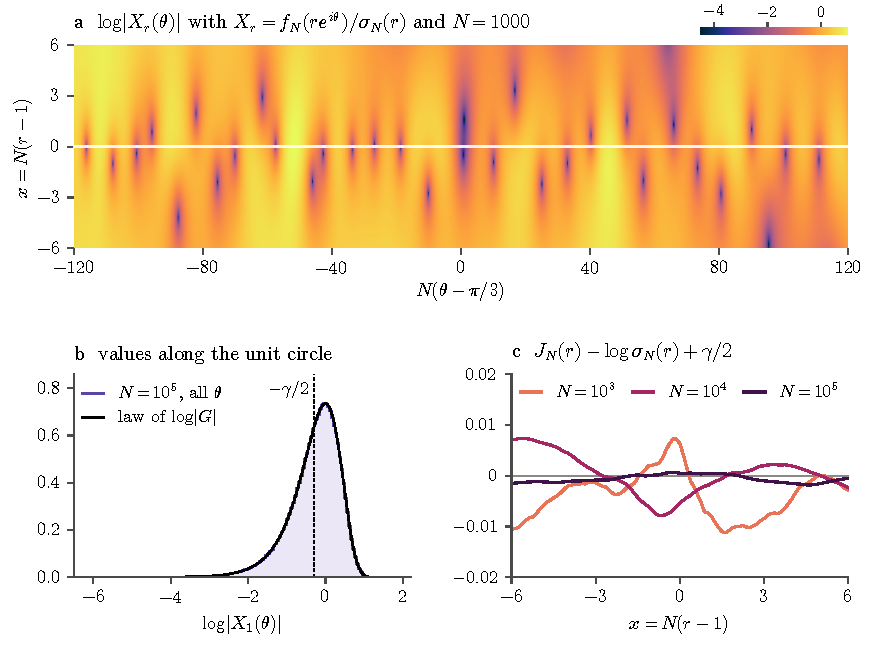
\includegraphics[width=\textwidth]{figures/explanatory/angular-logarithm.pdf}
\caption{The angular logarithm for one sequence near $e^{i\pi/3}$, with the
zeros as dark spots (a), its distribution (b), and its centered mean at
three degrees (c).}
\label{fig:angular-logarithm}
\end{figure}


\subsection{One- and two-point bounds}
\label{sec:h1-rademacher}
We show that, for radii $r,s\in[1-K/N,1+K/N]$ and for angles $\theta,\phi$
outside small exceptional sets, the probabilities that $X_r(\theta)$ lies
in a disk centered at $0$ and that $(X_r(\theta),X_s(\phi))$ lies in a
product of two such disks differ by $O_K(N^{-1/2})$ from those for one and
for two independent copies of $G$. Summation by parts shows that the
covariance matrices are close to $\tfrac12I$, Rai\v{c}'s theorem and an
interpolation of densities compare the laws with that of $G$, and we then
deduce bounds for the mean and the variance of the angular occupation of
a disk.

By the definition of $X_r$,
\[
 \begin{pmatrix}\Re X_r(\theta)\\ \Im X_r(\theta)\end{pmatrix}
 =\sum_{k=0}^N\epsilon_k\frac{r^k}{\sigma_N(r)}
 \begin{pmatrix}\cos(k\theta)\\ \sin(k\theta)\end{pmatrix}.
\]
Since the signs are independent with mean zero and variance one, the
covariance matrix of $(\Re X_r(\theta),\Im X_r(\theta))$ is given by
\[
 V(r,\theta)=\frac1{\sigma_N(r)^2}\sum_{k=0}^Nr^{2k}
 \begin{pmatrix}
 \cos^2(k\theta)&\cos(k\theta)\sin(k\theta)\\
 \cos(k\theta)\sin(k\theta)&\sin^2(k\theta)
 \end{pmatrix}.
\]
For two points, the covariance matrix of
$(\Re X_r(\theta),\Im X_r(\theta),\Re X_s(\phi),\Im X_s(\phi))$ is the
$4\times4$ matrix
\[
 \begin{pmatrix}
 V(r,\theta)&V(r,s,\theta,\phi)\\
 V(r,s,\theta,\phi)^T&V(s,\phi)
 \end{pmatrix},
\]
where
\[
 V(r,s,\theta,\phi)=\frac1{\sigma_N(r)\sigma_N(s)}\sum_{k=0}^N(rs)^k
 \begin{pmatrix}
 \cos(k\theta)\cos(k\phi)&\cos(k\theta)\sin(k\phi)\\
 \sin(k\theta)\cos(k\phi)&\sin(k\theta)\sin(k\phi)
 \end{pmatrix},
\]
so that $V(r,\theta)=V(r,r,\theta,\theta)$.
By the product-to-sum identities with $x,y\in\{k\theta,k\phi\}$, and
since $\sigma_N(r)^2=\sum_{k=0}^Nr^{2k}$, we get
\begin{align*}
 V(r,\theta)&=\frac12I_2+\frac1{2\sigma_N(r)^2}\sum_{k=0}^Nr^{2k}
 \begin{pmatrix}
 \cos(2k\theta)&\sin(2k\theta)\\
 \sin(2k\theta)&-\cos(2k\theta)
 \end{pmatrix},\\
 V(r,s,\theta,\phi)&=\frac1{2\sigma_N(r)\sigma_N(s)}\sum_{k=0}^N(rs)^k\\
 &\quad\times
 \begin{pmatrix}
 \cos(k(\theta-\phi))+\cos(k(\theta+\phi))&
 \sin(k(\theta+\phi))-\sin(k(\theta-\phi))\\
 \sin(k(\theta+\phi))+\sin(k(\theta-\phi))&
 \cos(k(\theta-\phi))-\cos(k(\theta+\phi))
 \end{pmatrix}.
\end{align*}
In terms of the rotation and the reflection
\begin{equation}
 R(\psi)=\begin{pmatrix}\cos\psi&-\sin\psi\\ \sin\psi&\cos\psi\end{pmatrix},
 \qquad
 F(\psi)=\begin{pmatrix}\cos\psi&\sin\psi\\ \sin\psi&-\cos\psi\end{pmatrix},
 \label{eq:rotation-reflection}
\end{equation}
the matrix summands are $F(2k\theta)$ and
$\Theta_k=R(k(\theta-\phi))+F(k(\theta+\phi))$, so that
\begin{align*}
 V(r,\theta)&=\frac12I_2+\frac1{2\sigma_N(r)^2}\sum_{k=0}^Nr^{2k}F(2k\theta),\\
 V(r,s,\theta,\phi)&=\frac1{2\sigma_N(r)\sigma_N(s)}\sum_{k=0}^N(rs)^k\Theta_k.
\end{align*}
The oscillatory sums are small unless $2\theta$, $2\phi$, $\theta-\phi$ or
$\theta+\phi$ is close to $2\pi\mathbb Z$, and we remove these angles.

For one point, we remove the set
$\operatorname{dist}(\theta,\pi\mathbb Z)<N^{-1/2}$: two arcs of length
$2N^{-1/2}$, of normalized measure
$4N^{-1/2}/(2\pi)=2N^{-1/2}/\pi\le2N^{-1/2}$. Every retained angle
satisfies
$\operatorname{dist}(2\theta,2\pi\mathbb Z)=2\operatorname{dist}(\theta,\pi\mathbb Z)\ge2N^{-1/2}$.
For two points, we remove this set in each coordinate, and the sets
$\operatorname{dist}(\theta\mp\phi,2\pi\mathbb Z)<N^{-1/2}$, each an arc of
$\theta$ of normalized length $N^{-1/2}/\pi$ for fixed $\phi$. The removed
part of the angular square has measure at most
$2N^{-1/2}+2N^{-1/2}+2N^{-1/2}/\pi\le10N^{-1/2}$.

The entries of these matrices are real and imaginary parts of weighted
exponential sums, which we bound by summation by parts.
Let $r,s\in[1-K/N,1+K/N]$, $N\ge2K$ and $\beta\in\{0,1,2\}$, and for
$\operatorname{dist}(\psi,2\pi\mathbb Z)>0$ set
\[
 b_k=(rs)^k(k/N)^\beta,\qquad S_\ell(\psi)=\sum_{k=0}^\ell e^{ik\psi},
\]
where $(k/N)^0=1$, including $k=0$, and $S_{-1}(\psi)=0$.
Summing the geometric series, and since
$|1-e^{i\psi}|=2|\sin(\psi/2)|\ge2\operatorname{dist}(\psi,2\pi\mathbb Z)/\pi$,
we get
\[
 S_\ell(\psi)=\frac{1-e^{i(\ell+1)\psi}}{1-e^{i\psi}},\qquad
 |S_\ell(\psi)|\le\frac2{|1-e^{i\psi}|}
 \le\frac\pi{\operatorname{dist}(\psi,2\pi\mathbb Z)}.
\]
Summation by parts yields
\[
 \sum_{k=0}^Nb_ke^{ik\psi}
 =\sum_{k=0}^Nb_k\bigl(S_k(\psi)-S_{k-1}(\psi)\bigr)
 =b_NS_N(\psi)+\sum_{k=0}^{N-1}(b_k-b_{k+1})S_k(\psi).
\]
For $\beta=0$ the weights are geometric. For $\beta>0$ we have $b_0=0$
and the ratios $b_{k+1}/b_k=(rs)(1+1/k)^\beta$, $k\ge1$, are
nonincreasing, so the weights first increase and then decrease (either
part may be empty). Let $b_*=\max_{k\le N}b_k$. The variation of such
weights is the rise from $b_0$ to $b_*$ plus the fall from $b_*$ to
$b_N$, and $b_k\le(rs)^k\le\max(1,rs)^N$ with $rs\le(1+K/N)^2$, so that
\begin{align*}
 b_*&\le(1+K/N)^{2N}\le e^{2K},\\
 \sum_{k=0}^{N-1}|b_{k+1}-b_k|&=2b_*-b_0-b_N,\\
 b_N+\sum_{k=0}^{N-1}|b_{k+1}-b_k|
 &\le b_0+b_N+2b_*\le4e^{2K}.
\end{align*}
Consequently, since $4\pi\le10e^{2K}$ for $K\ge2$,
\begin{equation}
 \begin{aligned}
 \left|N^{-1}\sum_{k=0}^N(rs)^k(k/N)^\beta e^{ik\psi}\right|
 &\le\frac\pi{N\operatorname{dist}(\psi,2\pi\mathbb Z)}
       \left(b_N+\sum_{k=0}^{N-1}|b_{k+1}-b_k|\right)\\
 &\le\frac{4\pi e^{2K}}{N\operatorname{dist}(\psi,2\pi\mathbb Z)}
 \le\frac{10e^{4K}}{N\operatorname{dist}(\psi,2\pi\mathbb Z)}.
 \end{aligned}                                      \label{eq:layer2-abel}
\end{equation}
We keep the larger constant $10e^{4K}$, from which the later bounds are
computed.

If $N\ge2K$ and $r\in[1-K/N,1+K/N]$, then each term of $\sigma_N(r)^2$
satisfies $e^{-4K}\le(1-K/N)^{2N}\le r^{2k}\le(1+K/N)^{2N}\le e^{2K}$,
since $\log(1-x)\ge-2x$ for $0\le x\le K/N\le1/2$. Summing the $N+1$
terms, we get the radial bounds
\begin{equation}
 Ne^{-4K}\le(N+1)e^{-4K}\le\sigma_N(r)^2\le(N+1)e^{2K}\le2Ne^{2K}.
 \label{eq:radial-bounds}
\end{equation}

The entries of $R(\psi)$ and $F(\psi)$ are $\pm\cos\psi$ and
$\pm\sin\psi$. Hence every entry of $V(r,\theta)-\tfrac12I_2$ is
$N/(2\sigma_N(r)^2)$ times $\pm$ the real or imaginary part of the sum in
\eqref{eq:layer2-abel} with $s=r$, $\beta=0$ and $\psi=2\theta$, and every
entry of $V(r,s,\theta,\phi)$ is $N/(2\sigma_N(r)\sigma_N(s))$ times the
sum of two such terms, with $\beta=0$ and $\psi=\theta\mp\phi$.
At the retained angles, by \eqref{eq:layer2-abel} and the lower bound in
\eqref{eq:radial-bounds}, these entries are at most, in absolute value,
\begin{equation}
 \begin{aligned}
 \frac N{2\sigma_N(r)^2}
 \left|\frac1N\sum_{k=0}^Nr^{2k}e^{2ik\theta}\right|
 &\le\frac{e^{4K}}2\cdot\frac{10e^{4K}}{N\cdot2N^{-1/2}}
 \le10e^{8K}N^{-1/2},\\
 \frac N{2\sigma_N(r)\sigma_N(s)}\sum_{\pm}
 \left|\frac1N\sum_{k=0}^N(rs)^ke^{ik(\theta\pm\phi)}\right|
 &\le\frac{e^{4K}}2\cdot2\cdot\frac{10e^{4K}}{N\cdot N^{-1/2}}
 =10e^{8K}N^{-1/2}.
 \end{aligned}\label{eq:covariance-entries}
\end{equation}
The first bound also holds for $V(s,\phi)-\tfrac12I_2$. The operator
norm of a $d\times d$ matrix is at most $d$ times its largest entry, so
at the retained angles $V(r,\theta)-\tfrac12I_2$ and the $4\times4$
covariance matrix minus $\tfrac12I_4$ have norm at most
$40e^{8K}N^{-1/2}$. From now on $N\ge(160e^{8K})^2$, so that this norm is
at most $1/4$ and every eigenvalue lies in $[1/4,3/4]$.

Rai\v{c}'s theorem \cite[Theorem 1.1]{Raic2019} states that, for
independent centered real vectors $Y_k$ with total covariance $I_d$ and a
measurable convex set $D$,
\[
 \left|\Prob\!\left(\sum_kY_k\in D\right)-\Prob(G_d\in D)\right|
 \le(42d^{1/4}+16)\sum_k\mathbb E\|Y_k\|^3,
\]
where $G_d$ is standard Gaussian in $\mathbb R^d$. For a covariance
matrix $\Sigma$ we write $G_\Sigma$ for a centered Gaussian vector with
covariance $\Sigma$, so that $G_d=G_{I_d}$; distances and entropies
between such vectors are those of their laws.
For two points, the summands and their covariance are
\[
 u_k=\begin{pmatrix}
 r^k\cos(k\theta)/\sigma_N(r)\\r^k\sin(k\theta)/\sigma_N(r)\\
 s^k\cos(k\phi)/\sigma_N(s)\\s^k\sin(k\phi)/\sigma_N(s)
 \end{pmatrix},\qquad
 \Sigma=\sum_{k=0}^Nu_ku_k^T,
\]
so that $\sum_{k=0}^N\epsilon_ku_k$ is the vector
$(\Re X_r(\theta),\Im X_r(\theta),\Re X_s(\phi),\Im X_s(\phi))^T$, whose
covariance $\Sigma$ is the $4\times4$ matrix above.
Let $Y_k=\epsilon_k\Sigma^{-1/2}u_k$. These are independent and centered,
since $\mathbb E\epsilon_k=0$ and $\mathbb E\epsilon_k^2=1$, and
$\|Y_k\|\le\|\Sigma^{-1/2}\|\|u_k\|\le2\|u_k\|$, since every eigenvalue of
$\Sigma$ is at least $1/4$. By $r^{2k},s^{2k}\le e^{2K}$ and the lower
bound in \eqref{eq:radial-bounds},
\begin{align*}
 \sum_{k=0}^N\mathbb E[Y_kY_k^T]
 &=\Sigma^{-1/2}\left(\sum_{k=0}^Nu_ku_k^T\right)\Sigma^{-1/2}
 =I_4,\\
 \|u_k\|^2
 &=\frac{r^{2k}}{\sigma_N(r)^2}+\frac{s^{2k}}{\sigma_N(s)^2}
 \le\frac{2e^{6K}}N,\\
 \sum_{k=0}^N\mathbb E\|Y_k\|^3
 &\le(N+1)\left(\frac{2\sqrt2e^{3K}}{\sqrt N}\right)^3
 \le32\sqrt2\,e^{9K}N^{-1/2}
 <46e^{9K}N^{-1/2}.
\end{align*}
For one point we use the first two coordinates, with
$\Sigma=V(r,\theta)$, and get the smaller bound
\[
 \|u_k\|^2=\frac{r^{2k}}{\sigma_N(r)^2}\le\frac{e^{6K}}N,\qquad
 \sum_{k=0}^N\mathbb E\|Y_k\|^3
 \le(N+1)\left(\frac{2e^{3K}}{\sqrt N}\right)^3
 \le16e^{9K}N^{-1/2}.
\]
Disks, products of disks and their images under whitening are
measurable and convex.

To compare $G_\Sigma$ with $G_{I_d/2}$, where $d=2$ or $4$, let
$\Delta=\Sigma-\tfrac12I_d$, so that $\|\Delta\|\le40e^{8K}N^{-1/2}\le1/4$,
and let $p_\lambda$ be the centered Gaussian
density with covariance $\Sigma_\lambda=\tfrac12I_d+\lambda\Delta$,
$0\le\lambda\le1$, whose eigenvalues lie in $[1/4,3/4]$. Then
\begin{align}
 \partial_\lambda p_\lambda(x)
 &=\frac{p_\lambda(x)}2\left\{
   x^T\Sigma_\lambda^{-1}\Delta\Sigma_\lambda^{-1}x-\operatorname{tr}(\Sigma_\lambda^{-1}\Delta)
   \right\},\nonumber\\
 \int_{\mathbb R^d}|\partial_\lambda p_\lambda(x)|\dd x
 &=\frac12\,\mathbb E\bigl|G_d^T\Sigma_\lambda^{-1/2}\Delta\Sigma_\lambda^{-1/2}G_d
   -\operatorname{tr}(\Sigma_\lambda^{-1/2}\Delta\Sigma_\lambda^{-1/2})\bigr|\nonumber\\
 &\le\frac{\sqrt{2d}}2\|\Sigma_\lambda^{-1/2}\Delta\Sigma_\lambda^{-1/2}\|
 \le2\sqrt{2d}\,\|\Delta\|,\nonumber\\
 \operatorname{TV}\bigl(G_\Sigma,G_{I_d/2}\bigr)
 &\le\frac12\int_0^1\int_{\mathbb R^d}|\partial_\lambda p_\lambda(x)|\dd x\dd\lambda
 \le\sqrt{2d}\,\|\Delta\|
 \le320e^{8K}N^{-1/2}.\label{eq:tv-circular}
\end{align}
The four lines of \eqref{eq:tv-circular} hold for these reasons.
\begin{enumerate}
\item The derivative uses
$\partial_\lambda\log\det\Sigma_\lambda=\operatorname{tr}(\Sigma_\lambda^{-1}\Delta)$
and
$\partial_\lambda\Sigma_\lambda^{-1}=-\Sigma_\lambda^{-1}\Delta\Sigma_\lambda^{-1}$.
\item The change of variables $x\mapsto\Sigma_\lambda^{-1/2}x$ carries
$p_\lambda$ to the law of $G_d$.
\item In an eigenbasis of $\Sigma_\lambda^{-1/2}\Delta\Sigma_\lambda^{-1/2}$,
with eigenvalues $a_1,\ldots,a_d$, the quadratic form minus the trace is
$\sum_ia_i(g_i^2-1)$ with independent standard real Gaussian $g_i$. It has
mean zero and variance
$2\sum_ia_i^2\le2d\|\Sigma_\lambda^{-1/2}\Delta\Sigma_\lambda^{-1/2}\|^2$,
so by Cauchy--Schwarz its mean absolute value is at most $\sqrt{2d}$ times
this norm, which is at most $4\|\Delta\|$ since
$\|\Sigma_\lambda^{-1}\|\le4$.
\item Total variation is half the $L^1$ distance,
$p_1-p_0=\int_0^1\partial_\lambda p_\lambda\dd\lambda$, and
$\sqrt{2d}\le2\sqrt2\le8$ for $d\le4$.
\end{enumerate}
The same computation gives, for positive-definite $\Sigma_0,\Sigma_1$ in
dimension $d$ such that every $\Sigma_0+\lambda(\Sigma_1-\Sigma_0)$,
$0\le\lambda\le1$, has least eigenvalue at least $\mu>0$,
$\operatorname{TV}(G_{\Sigma_1},G_{\Sigma_0})\le\sqrt{2d}\,\|\Sigma_1-\Sigma_0\|/(4\mu)$,
since the norm of $\Sigma_\lambda^{-1/2}(\Sigma_1-\Sigma_0)\Sigma_\lambda^{-1/2}$
is at most $\|\Sigma_1-\Sigma_0\|/\mu$.

Let $F_G(t)=\Prob(|G|\le t)=1-e^{-t^2}$, and for $t,t'\ge0$ let $D$ be
the disk $\{x\in\mathbb R^2:x_1^2+x_2^2\le t^2\}$ when $d=2$ and the
product of disks
$\{x\in\mathbb R^4:x_1^2+x_2^2\le t^2,\ x_3^2+x_4^2\le t'^2\}$ when $d=4$.
Since $\sum_k\epsilon_ku_k=\Sigma^{1/2}\sum_kY_k$ and $\Sigma^{1/2}G_d$
has the law of $G_\Sigma$, we have
$\Prob(\sum_k\epsilon_ku_k\in D)=\Prob(\sum_kY_k\in\Sigma^{-1/2}D)$ and
$\Prob(G_\Sigma\in D)=\Prob(G_d\in\Sigma^{-1/2}D)$. Hence, by Rai\v{c}'s
theorem with the third-moment bounds above and by \eqref{eq:tv-circular},
at retained angles and pairs,
\begin{align}
 &\bigl|\Prob\bigl(\textstyle\sum_k\epsilon_ku_k\in D\bigr)-\Prob(G_{I_d/2}\in D)\bigr|
 \nonumber\\
 &\qquad\le\bigl|\Prob\bigl(\textstyle\sum_kY_k\in\Sigma^{-1/2}D\bigr)
     -\Prob(G_d\in\Sigma^{-1/2}D)\bigr|
 +\bigl|\Prob(G_\Sigma\in D)-\Prob(G_{I_d/2}\in D)\bigr|
 \nonumber\\
 &\qquad\le(42d^{1/4}+16)\cdot46e^{9K}N^{-1/2}+320e^{8K}N^{-1/2}
 \le C(K)N^{-1/2}.\label{eq:point-bounds}
\end{align}
For $d=4$ the left-hand side is
$|\Prob(|X_r(\theta)|\le t,|X_s(\phi)|\le t')-F_G(t)F_G(t')|$, since the
two coordinate pairs of $G_{I_4/2}$ are independent copies of $G$, and
for $d=2$ it is $|\Prob(|X_r(\theta)|\le t)-F_G(t)|$.

Let $A_t=\mu\{\theta:|X_r(\theta)|\le t\}$ be the angular occupation.
By Tonelli's theorem,
\begin{align*}
 \mathbb EA_t&=\int\Prob(|X_r(\theta)|\le t)\dd\mu(\theta),\\
 \mathbb EA_t^2&=\int\!\!\int
   \Prob(|X_r(\theta)|\le t,|X_r(\phi)|\le t)\dd\mu(\theta)\dd\mu(\phi).
\end{align*}
On the removed sets, of measures at most $2N^{-1/2}$ and $10N^{-1/2}$, the
integrands differ from $F_G(t)$ and $F_G(t)^2$ by at most one; elsewhere
we use \eqref{eq:point-bounds}, with $s=r$ and $t'=t$ for the pairs.
Hence, uniformly for $t\ge0$, since $0\le\mathbb EA_t+F_G(t)\le2$,
\begin{align}
 |\mathbb EA_t-F_G(t)|&\le2N^{-1/2}+C(K)N^{-1/2}\le C(K)N^{-1/2},\nonumber\\
 |\mathbb EA_t^2-F_G(t)^2|&\le10N^{-1/2}+C(K)N^{-1/2}\le C(K)N^{-1/2},\nonumber\\
 \operatorname{Var}(A_t)
 &=\mathbb EA_t^2-F_G(t)^2-(\mathbb EA_t-F_G(t))(\mathbb EA_t+F_G(t))
 \nonumber\\
 &\le|\mathbb EA_t^2-F_G(t)^2|
       +|\mathbb EA_t-F_G(t)|\,|\mathbb EA_t+F_G(t)|
 \le C(K)N^{-1/2}.\label{eq:occupation-bounds}
\end{align}
The two-point argument also permits different radii and different disk
thresholds.

\subsection{Logarithmic integrability and angular energy}\label{sec:log-integrability}
The normalized Fourier coefficients satisfy
$\sum_{k=0}^N|r^k/\sigma_N(r)|^2=1$, which is the normalization in
$L^2(\Omega\times\mathbb T)$ of Corollary~1.2 of Nazarov--Nishry--Sodin
\cite{NNS2013}. By that corollary,
\begin{equation}
 \mathbb E\int |\log|X_r||^p\dd\mu\le(C_*p)^{6p},\qquad p\ge1,
                                                        \label{eq:layer2-nns}
\end{equation}
where $C_*\ge1$ is an absolute constant; zeros on the circle give only
integrable logarithmic singularities. By Parseval's identity, for every
choice of signs, the angular energy is
\begin{equation}
 \int|X_r|^2\dd\mu=\frac1{\sigma_N(r)^2}\sum_{k=0}^N\epsilon_k^2r^{2k}=1.
                                                        \label{eq:layer2-energy}
\end{equation}

We clip the logarithm at $\pm T$, control the clipped integral by the
occupation bounds, and control the two tails by the logarithmic moments
and the angular energy. Table~\ref{tab:clipping-level} lists what depends
on $T$.
\begin{table}[ht]
\centering
\small
\setlength{\tabcolsep}{4pt}
\begin{tabular}{@{}llll@{}}
\toprule
Quantity & Bound & At $T=c\log N$ & Requirement\\
\midrule
Gaussian mass of $\{|z|\le e^{-T}\}$ & $F_G(e^{-T})\le e^{-2T}$ & $N^{-2c}$ & tends to zero\\
Chebyshev bound for $A_{e^{-T}}$ & $C(K)N^{-1/2}e^{4T}$ & $C(K)N^{4c-1/2}$ & summable in $j$\\
Lower tail ($e^{-2T}\ge N^{-1/2}$) & order $(\log N)^7e^{-2T}$ & $(\log N)^7N^{-2c}$ & tends to zero\\
\bottomrule
\end{tabular}
\caption{The quantities in Lemma~\ref{lem:clipping} that depend on the
clipping level $T=c\log N$, for signs; the last row needs $c\le1/4$.
At $N=j^8$ the second is $C(K)j^{32c-4}$, summable when $c<3/32$.}
\label{tab:clipping-level}
\end{table}
Any $c$ in $(0,3/32)$ would do. By H\"older's inequality in
Theorem~\ref{thm:T1} the lower tail is of order $e^{-2T}$, up to the
logarithmic factor, so a larger $c$ gives a smaller error and a larger
failure probability. We take $c=1/32$: then $T=(1/32)\log N$,
$e^{-2T}=N^{-1/16}\ge N^{-1/2}$, the lower tail is
$(\log N)^7N^{-1/16}$, the error term of
Theorem~\ref{thm:sign-logarithms}, and
$N^{-1/2}e^{4T}=N^{-3/8}$, which is $j^{-3}$ at $N=j^8$. This failure
probability stays summable when $C(K)$ grows like a small power of $N$,
as in Section~\ref{sec:log-rate}.
We state the argument for coefficients that need not be signs, for use in
Section~\ref{sec:layer2-models}.

Theorem~\ref{thm:T1}, which we apply below, uses two facts about the
standard complex Gaussian variable $G$. For every $T\ge0$, since
$F_G(e^{-\tau})\le e^{-2\tau}$ and
$\Prob(|G|>e^\tau)\le e^{-2\tau}\mathbb E|G|^2=e^{-2\tau}$,
\begin{equation}
 \int_T^\infty\Prob(|G|<e^{-\tau})\dd\tau\le\tfrac12e^{-2T},\qquad
 \int_T^\infty\Prob(|G|>e^\tau)\dd\tau\le\tfrac12e^{-2T}.
 \label{eq:gaussian-log-tails}
\end{equation}
Since $|G|^2$ has the exponential distribution with mean one, the
classical integral for Euler's constant gives
\begin{equation}
 \mathbb E\log|G|=\frac12\,\mathbb E\log(|G|^2)
 =\frac12\int_0^\infty e^{-y}\log y\dd y
 =-\frac\gamma2.
 \label{eq:euler-centering}
\end{equation}

\begin{lemma}[Clipping]\label{lem:clipping}
Let $N\ge e$ and $r>0$, and let $X_r$ and $A_t$ be defined as above for a
random polynomial $f_N$ whose coefficients need not be signs.
Let $H\ge0$, $C>0$ and $B_E>0$ be constants and $E$ an event such that,
for all $t\ge0$ and $p\ge1$,
\begin{gather*}
 |\mathbb EA_t-F_G(t)|\le HN^{-1/2},\qquad
 \operatorname{Var}(A_t)\le HN^{-1/2},\\
 \int_E\int|\log|X_r||^p\dd\mu\dd\Prob\le(Cp)^{6p},
\end{gather*}
and $\int|X_r|^2\dd\mu\le B_E$ on $E$. Let $T=(1/32)\log N$ and
\begin{align*}
 \varepsilon&=N^{-1/16}(\log N)^7+2HTN^{-1/2}\\
 &\quad+e^{1/2}(4eC)^6(2N^{-1/16}+HN^{-1/2})(\log N)^7+(B_E/2+1)N^{-1/16}\\
 &\le\bigl(2+2e^{1/2}(4eC)^6+B_E/2\bigr)N^{-1/16}(\log N)^7\\
 &\quad+\bigl(\tfrac1{16}+e^{1/2}(4eC)^6\bigr)HN^{-1/2}(\log N)^7.
\end{align*}
Then
\begin{align*}
 &\Prob\{|J_N(r)-\log\sigma_N(r)+\gamma/2|>\varepsilon\}\\
 &\qquad\le HN^{-3/8}+N^{-12}+\frac{H}{256}N^{-3/8}(\log N)^{-12}
 +\Prob(E^c).
\end{align*}
\end{lemma}

\begin{proof}
This is Theorem~\ref{thm:T1} in the variant form given at the end of its
statement, with $X=X_r$,
$d_1=v=HN^{-1/2}$, $\beta=6$, $E_H=E$, $T=(1/32)\log N$,
$u=N^{-1/16}(\log N)^7$, $b=N^{-1/16}$, $q=\lceil\log N\rceil$ and
$\lambda=(2e\log N/q)^6\log N$. Its hypotheses hold, since the
occupation bounds of the lemma are the bounds on $\mathbb EA_t$ and
$\operatorname{Var}(A_t)$ of that form, the moment bound of the lemma
is \eqref{eq:event-log-moment-bound} with $E_H=E$ and $\beta=6$, and
$\int|X_r|^2\dd\mu\le B_E$ on $E$.
For $N\ge e$ we have $\log N\le q\le\log N+1\le2\log N$, so that
$\lambda\ge e^6\log N>1$,
\[
 \lambda(2Cq)^6
 =\Bigl(\frac{2e\log N}q\Bigr)^6(\log N)(2Cq)^6
 =(4eC)^6(\log N)^7
\]
and
\[
 \lambda^{-2q}
 =\left[\left(\frac q{2e\log N}\right)^{12}(\log N)^{-2}\right]^q
 \le\bigl[e^{-12}(\log N)^{-2}\bigr]^q
 \le N^{-12},
\]
where the last two steps use $q\le2\log N$, $\log N\ge1$ and
$q\ge\log N$. By the first identity, the Markov event for $W$ in the
proof of Theorem~\ref{thm:T1} is
$E\cap\{W>((4eC)^6(\log N)^7)^{2q}\}$, where
$W=\int|\log|X_r||^{2q}\dd\mu$.
Since $e^{-2T}=b=N^{-1/16}$, the base
$x=e^{-2T}+d_1+b=2N^{-1/16}+HN^{-1/2}$ satisfies $x\ge N^{-1}$, and
hence $x^{-1/(2q)}\le N^{1/(2q)}\le e^{1/2}$, since $q\ge\log N$, so that
\[
 x^{1-1/(2q)}\le e^{1/2}x=e^{1/2}(2N^{-1/16}+HN^{-1/2}),
\]
and the error $\eta_{\log}$ of \eqref{eq:T1-error} is at most
$\varepsilon$. The first three terms of \eqref{eq:T1-failure} are
$v/b^2=HN^{-1/2}N^{1/8}=HN^{-3/8}$, $\lambda^{-2q}\le N^{-12}$ and
$4T^2v/u^2=4HT^2N^{-3/8}(\log N)^{-14}=(H/256)N^{-3/8}(\log N)^{-12}$,
since $4T^2=(\log N)^2/256$, and $p_E+p_H$ is replaced by
$\Prob(E^c)$.
Since $J_N(r)-\log\sigma_N(r)=\int\log|X_r|\dd\mu$ and
$\mathbb E\log|G|=-\gamma/2$ by \eqref{eq:euler-centering}, this is the
bound of the lemma. The bound on $\varepsilon$ in the statement uses
$2TN^{-1/2}=\frac1{16}N^{-1/2}\log N\le\frac1{16}N^{-1/2}(\log N)^7$ and
$N^{-1/16}\le N^{-1/16}(\log N)^7$ for $N\ge e$, and keeps the terms with
$H$, which carry the factor $N^{-1/2}$, apart from the others.
\end{proof}

\begin{proof}[Proof of Theorem~\ref{thm:sign-logarithms}]
By \eqref{eq:occupation-bounds}, \eqref{eq:layer2-nns} and
\eqref{eq:layer2-energy}, Lemma~\ref{lem:clipping} applies with $H$ the
constant $C(K)$ of \eqref{eq:occupation-bounds}, $C=C_*$, $E=\Omega$ and
$B_E=1$.
Since $C_*$ is an absolute constant and $N^{-1/2}\le N^{-1/16}$, its
error $\varepsilon$ is at most $C(K)N^{-1/16}(\log N)^7$, and, since
$\Prob(E^c)=0$, its probability
bound is at most the right-hand side of
\eqref{eq:sign-log-concentration}.
All constants above depend only on $K$, and all bounds hold uniformly
for $r\in[1-K/N,1+K/N]$.
\end{proof}

\subsection{Radial mass and thin bands with high probability}

\begin{corollary}[Annular mass and thin bands]\label{cor:radial-probability}
Fix $K\ge2$ and $0<\kappa\le1/64$, and take $N$ sufficiently large.
Outside four events, each of probability at most the right-hand side of
\eqref{eq:sign-log-concentration},
\begin{equation}
 \frac{\#\{\alpha:||\alpha|-1|>K/N\}}N
 \le\frac{2\log2}{K}+C(K)N^{-1/16}(\log N)^7.
                                                        \label{eq:sign-annular-mass}
\end{equation}
Outside five further events of the same kind, for
$q=-1,0,1$,
\begin{equation}
 \left|\frac{\nu_N(1+qN^{-1-\kappa})}N-\frac12\right|
 \le2N^{-\kappa}+C(K)N^{\kappa-1/16}(\log N)^7.
                                                        \label{eq:sign-thin-band}
\end{equation}
\end{corollary}

By Theorem~\ref{thm:sign-logarithms}, the sum of the probabilities of
these nine exceptional events is summable at $N=j^8$.

\begin{proof}
We apply the deterministic Lemmas~\ref{lem:annular-mass}
and~\ref{lem:thin-band} outside the exceptional events of
Theorem~\ref{thm:sign-logarithms} at their radii; $f_N\ne0$ since
$f_N(0)=\epsilon_0\ne0$.

The four secant radii $r_i=1+x_i/N$ of Lemma~\ref{lem:annular-mass} with
$\eta=1/2$ lie in $[1-K/N,1+K/N]$. Outside the four logarithmic
exceptional events at these radii, the first hypothesis of that lemma
holds with $\varepsilon=C(K)N^{-1/16}(\log N)^7$, by
Theorem~\ref{thm:sign-logarithms}, and the second with
$D=K^2+e^{4K}/2$, by Lemma~\ref{lem:profile-rate}, since $|x_i|\le K$
and $N\ge2K$.
Therefore Lemma~\ref{lem:annular-mass} at $\eta=1/2$ and
$1/N\le N^{-1/16}(\log N)^7$, for $N\ge3$, yield
\begin{align*}
 \frac{\#\{\alpha:||\alpha|-1|>K/N\}}N
 &\le\frac{2\log2}K+\frac8K\Big(C(K)N^{-1/16}(\log N)^7
       +\frac{K^2+e^{4K}/2}N\Big)\\
 &\le\frac{2\log2}K+\frac8K\Big(C(K)+K^2+\frac{e^{4K}}2\Big)
       N^{-1/16}(\log N)^7\\
 &\le\frac{2\log2}{K}+C(K)N^{-1/16}(\log N)^7,
\end{align*}
which is \eqref{eq:sign-annular-mass}.

The five radii $1+qN^{-1-\kappa}$, $q=-2,\dots,2$, lie in the same
annulus, since $|qN^{-1-\kappa}|\le2N^{-1-\kappa}\le K/N$.
Outside the five logarithmic exceptional events at these radii,
Lemma~\ref{lem:thin-band} applies with
$\varepsilon=C(K)N^{-1/16}(\log N)^7$ (and $N\ge4$), and bounds the
left-hand side of \eqref{eq:sign-thin-band} by
$2N^{-\kappa}+4C(K)N^{-1/16}(\log N)^7N^{\kappa}
=2N^{-\kappa}+4C(K)N^{\kappa-1/16}(\log N)^7$.
Both terms tend to zero, since $\kappa\le1/64<1/16$.
\end{proof}

Figure~\ref{fig:annulus} compares the fraction of roots outside the
annulus with $2\log2/K$, the part of \eqref{eq:sign-annular-mass} that
does not tend to zero.
Panel (a) also shows the limit $1-\{\Phi(K)-\Phi(-K)\}$ of the fraction,
and panel (b) shows $K$ times its difference from this limit, with
pointwise 95\% bootstrap bands, both over 77 sequences.

\begin{figure}[t]
\centering
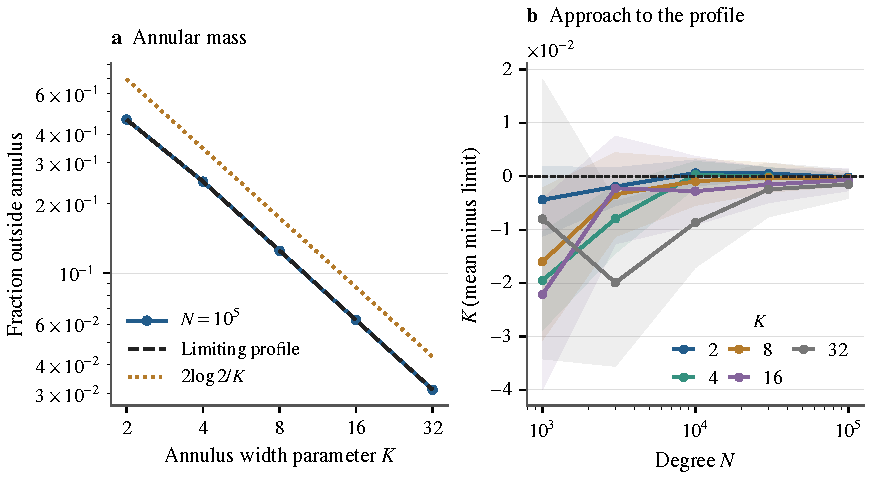
\includegraphics[width=\textwidth]{../numerics/publication/figures/annulus.pdf}
\caption{The fraction of zeros outside the annulus of width $K/N$.}
\label{fig:annulus}
\end{figure}

